\documentclass[acmsmall]{acmart}

\usepackage{array}
\usepackage{tabularx}
% \usepackage{amssymb}
\usepackage{algorithm}
\usepackage{algpseudocode}

\newcommand{\yes}{\(\checkmark\)}
\newcommand{\no}{\(\times\)}

\newcolumntype{L}{>{\raggedright\arraybackslash}X}

%%
%% \BibTeX command to typeset BibTeX logo in the docs
\AtBeginDocument{%
  \providecommand\BibTeX{{%
    Bib\TeX}}}

%% Rights management information.  This information is sent to you
%% when you complete the rights form.  These commands have SAMPLE
%% values in them; it is your responsibility as an author to replace
%% the commands and values with those provided to you when you
%% complete the rights form.
\setcopyright{acmlicensed}
\copyrightyear{2026}
\acmYear{2026}
\acmDOI{XXXXXXX.XXXXXXX}
%% These commands are for a PROCEEDINGS abstract or paper.
\acmConference[Conference acronym 'XX]{Make sure to enter the correct
  conference title from your rights confirmation email}{June 03--05,
  2018}{Woodstock, NY}
%%
%%  Uncomment \acmBooktitle if the title of the proceedings is different
%%  from ``Proceedings of ...''!
%%
%%\acmBooktitle{Woodstock '18: ACM Symposium on Neural Gaze Detection,
%%  June 03--05, 2018, Woodstock, NY}
\acmISBN{978-1-4503-XXXX-X/2018/06}



%%
%% Submission ID.
%% Use this when submitting an article to a sponsored event. You'll
%% receive a unique submission ID from the organizers
%% of the event, and this ID should be used as the parameter to this command.
%%\acmSubmissionID{123-A56-BU3}

%%
%% For managing citations, it is recommended to use bibliography
%% files in BibTeX format.
%%
%% You can then either use BibTeX with the ACM-Reference-Format style,
%% or BibLaTeX with the acmnumeric or acmauthoryear sytles, that include
%% support for advanced citation of software artefact from the
%% biblatex-software package, also separately available on CTAN.
%%
%% Look at the sample-*-biblatex.tex files for templates showcasing
%% the biblatex styles.
%%
%%
%% The majority of ACM publications use numbered citations and
%% references.  The command \citestyle{authoryear} switches to the
%% "author year" style.
%%
%% If you are preparing content for an event
%% sponsored by ACM SIGGRAPH, you must use the "author year" style of
%% citations and references.
%% Uncommenting
%% the next command will enable that style.
%%\citestyle{acmauthoryear}


%%
%% end of the preamble, start of the body of the document source.
\begin{document}
\raggedbottom

%%
%% The "title" command has an optional parameter,
%% allowing the author to define a "short title" to be used in page headers.
\title{ML-based Deep Bitstream Inspection for
Serverless FPGAs}

%%
%% The "author" command and its associated commands are used to define
%% the authors and their affiliations.
%% Of note is the shared affiliation of the first two authors, and the
%% "authornote" and "authornotemark" commands
%% used to denote shared contribution to the research.
\author{Santiago de Heredia}
\email{sdeheredia@ethz.ch}
\affiliation{%
  \institution{Systems Group, ETH Zurich}
  \city{Zurich}
  \country{Switzerland}
}

\author{Maximilian J. Heer}
\email{maximilian.heer@inf.ethz.ch}
\affiliation{%
  \institution{Systems Group, ETH Zurich}
  \city{Zurich}
  \country{Switzerland}
}

\author{Gustavo Alonso}
\email{alonso@inf.ethz.ch}
\affiliation{%
  \institution{Systems Group, ETH Zurich}
  \city{Zurich}
  \country{Switzerland}
}

%%
%% By default, the full list of authors will be used in the page
%% headers. Often, this list is too long, and will overlap
%% other information printed in the page headers. This command allows
%% the author to define a more concise list
%% of authors' names for this purpose.
\renewcommand{\shortauthors}{de Heredia et al.}

%%
%% The abstract is a short summary of the work to be presented in the
%% article.
\begin{abstract}
    Cloud and serverless FPGA platforms expose reconfigurable fabric to user-submitted designs, creating risks from malicious circuits such as ring oscillators. Existing machine-learning approaches typically inspect bitstreams offline in software. We instead study an on-FPGA checker that analyzes incoming partial bitstreams before reconfiguration. We generate benign Coyote and ring-oscillator bitstreams, convert them into fixed-size byte-image tensors, train a quantized CNN, and synthesize it using hls4ml. Our selected $256^2$-input, seven-layer model achieves 88.5\% F1 and 95.1\% ROC AUC. Its estimated preprocessing and inference latency is 3.35\,ms, while the routed checker uses 4.47\% of LUTs, 17.86\% of BRAM, 1.15\% of URAM, and 14.72\% of DSPs on an Alveo U55C. These results demonstrate the feasibility of an on-FPGA checker for detecting malicious bitstreams before partial reconfiguration.
    \end{abstract}
%%
%% The code below is generated by the tool at http://dl.acm.org/ccs.cfm.
%% Please copy and paste the code instead of the example below.
%%
\begin{CCSXML}
<ccs2012>
 <concept>
  <concept_id>10002978.10003014</concept_id>
  <concept_desc>Security and privacy~Systems security</concept_desc>
  <concept_significance>500</concept_significance>
 </concept>
 <concept>
  <concept_id>10010520.10010521.10010537.10003100</concept_id>
  <concept_desc>Computer systems organization~Cloud computing</concept_desc>
  <concept_significance>300</concept_significance>
 </concept>
 <concept>
  <concept_id>10010147.10010257</concept_id>
  <concept_desc>Computing methodologies~Machine learning</concept_desc>
  <concept_significance>300</concept_significance>
 </concept>
 <concept>
  <concept_id>10010147.10010257.10010293.10010294</concept_id>
  <concept_desc>Computing methodologies~Neural networks</concept_desc>
  <concept_significance>100</concept_significance>
 </concept>
</ccs2012>
\end{CCSXML}

\ccsdesc[500]{Security and privacy~Systems security}
\ccsdesc[300]{Computer systems organization~Cloud computing}
\ccsdesc[300]{Computing methodologies~Machine learning}
\ccsdesc[100]{Computing methodologies~Neural networks}

%%
%% Keywords. The author(s) should pick words that accurately describe
%% the work being presented. Separate the keywords with commas.
\keywords{cloud FPGA security, bitstream inspection, partial bitsreams, malicious circuit detection,
serverless FPGAs, partial reconfiguration, convolutional neural networks, ML for systems, hls4ml}
%% A "teaser" image appears between the author and affiliation
%% information and the body of the document, and typically spans the
%% page.

\received{TODO}
\received[revised]{TODO}
\received[accepted]{TODO}

%%
%% This command processes the author and affiliation and title
%% information and builds the first part of the formatted document.
\maketitle

\section{Introduction}
\label{sec:introduction}

Field-programmable gate arrays (FPGAs) are increasingly used as datacenter
accelerators because they combine programmability with high performance and
energy efficiency~\cite{caulfield2016cloud,bobda2022future}. Cloud and
serverless FPGA platforms extend this model by allowing users to deploy
hardware applications on shared infrastructure. Partial reconfiguration (PR)
makes this practical by loading user logic into a reconfigurable region while
the trusted FPGA shell remains active~\cite{korolija2020os,ramhorst2025coyote}.

This deployment model exposes shared FPGA resources to untrusted user logic.
Malicious circuits such as ring-oscillator (RO) arrays can generate sustained
switching activity, causing voltage drops, timing faults, and denial of
service~\cite{gnad2017voltage,la2021denial,provelengios2020power,
boutros2020neighbors}. Demonstrated attacks on cloud FPGA infrastructure
therefore motivate inspecting user bitstreams before partial
reconfiguration~\cite{la2021denial}.

Prior work has shown that machine-learning models can identify malicious
designs from bitstream-derived representations without fully reconstructing
their circuit semantics~\cite{rettkowski2019inspection,
chaudhuri2022detection,elnaggar2023learning,palumbo2022trojan}. However, these
approaches are commonly evaluated as offline software classifiers. A serverless
FPGA platform instead needs a checker that can operate within the deployment
path, retain useful detection quality, fit alongside platform and user logic,
and avoid dominating PR latency.

We investigate an \emph{on-FPGA checker} placed before partial
reconfiguration. The checker transforms the raw bytes of an incoming partial
bitstream into a fixed-size tensor, executes a quantized convolutional neural
network (CNN), and returns a suspiciousness score to the deployment logic.
We study this design in the context of Coyote, a datacenter-grade FPGA shell
supporting PR and multitenancy~\cite{ramhorst2025coyote}. We generate benign
Coyote application bitstreams and RO-based malicious bitstreams, train compact
CNNs, and synthesize selected models using
hls4ml~\cite{duarte2018fast,aarrestad2021fast}.

Our evaluation identifies a seven-layer CNN operating on a
$256 \times 256$ byte-image representation as the preferred deployment
point. The resulting checker provides useful detection at millisecond-scale
latency while leaving sufficient resources for the Coyote shell and user logic.
The broader design-space exploration shows that modest improvements in
software classification quality can require sharply higher on-chip memory and
latency, making larger models unsuitable for deployment.


This work makes three contributions:

\begin{itemize}
    \item We construct a dataset of benign Coyote partial bitstreams and
    RO-based malicious bitstreams across multiple floorplans and payload
    footprints.

    \item We develop an on-FPGA inspection pipeline combining deterministic
    byte-stream preprocessing, quantized CNN inference, and hls4ml synthesis.

    \item We evaluate detection quality, latency, and routed FPGA resource
    overhead together, identifying a practical deployment point for
    pre-reconfiguration inspection.
\end{itemize}

\section{Background, Threat Model, and Related Work}
\label{sec:background}

\subsection{Deployment Setting and Threat Model}
\label{sec:threat-model}

Serverless FPGA platforms allow users to deploy hardware accelerators on shared
reconfigurable infrastructure. Partial reconfiguration (PR) supports this model
by dividing the FPGA into a trusted static shell and one or more reconfigurable
regions containing user logic. The shell remains active while individual user
regions are reconfigured, allowing the platform to retain control over host
communication, memory, networking, and runtime services
\cite{korolija2020os,ramhorst2025coyote}.

This separation creates a security boundary. A user-submitted partial bitstream
is an untrusted input that directly determines the circuit instantiated inside a
reconfigurable region. Malicious circuits can exploit physical resources shared
across the device, including power delivery, thermal headroom, and timing
margins. We focus on ring-oscillator (RO) payloads, which produce sustained
switching activity and can induce voltage drops, timing faults, or denial of
service when instantiated at sufficient scale
\cite{gnad2017voltage,la2021denial,provelengios2020power,boutros2020neighbors}.

We consider an attacker who can submit a syntactically valid partial bitstream
for a user region. The bitstream contains an RO-based payload intended to pass
existing platform checks and stress shared physical resources after
configuration.

The defender places an on-FPGA checker before PR. The checker is intended to inspect the same buffered bitstream bytes that would subsequently be provided to
the PR controller. It produces a maliciousness score that the trusted deployment
logic converts into an allow or reject decision. A true positive blocks and logs
a suspicious bitstream. A false negative allows a malicious bitstream to be
configured, while a false positive rejects a benign accelerator.
\subsection{Existing Defenses and Research Gap}
\label{sec:related-work}
Existing defenses against malicious FPGA designs broadly fall into three
groups. Table~\ref{tab:defense-comparison} summarizes their relationship to this
work.

\begin{table*}[t]
  \caption{Comparison of malicious-bitstream detection approaches across
  deployment and implementation dimensions.}
  \label{tab:defense-comparison}
  \centering
  \footnotesize

  \renewcommand{\arraystretch}{1.18}
  \setlength{\tabcolsep}{4pt}
  \renewcommand{\tabularxcolumn}[1]{m{#1}}

  \begin{tabularx}{\textwidth}{
    @{}
    >{\raggedright\arraybackslash}m{0.15\textwidth}
    >{\raggedright\arraybackslash}m{0.16\textwidth}
    >{\centering\arraybackslash}m{0.095\textwidth}
    >{\centering\arraybackslash}m{0.085\textwidth}
    >{\centering\arraybackslash}m{0.105\textwidth}
    >{\centering\arraybackslash}m{0.095\textwidth}
    L
    @{}
  }
    \toprule

    \textbf{Approach}
      & \textbf{Detection basis}
      & \multicolumn{2}{c}{\textbf{Deployment}}
      & \multicolumn{2}{c}{\textbf{Properties}}
      & \textbf{Target} \\

    \cmidrule(lr){3-4}
    \cmidrule(lr){5-6}

    &
    & \shortstack[c]{\textbf{Deployment}\\\textbf{integrated}}
    & \shortstack[c]{\textbf{On-}\\\textbf{FPGA}}
    & \shortstack[c]{\textbf{No reverse}\\\textbf{engineering}}
    & \shortstack[c]{\textbf{Datacenter}\\\textbf{target}}
    & \\

    \midrule

    Platform checks
      & Provider-defined rules
      & \yes
      & \no
      & \yes
      & \yes
      & Cloud deployment \\

    \addlinespace[2pt]

    Structural scanning
      & Circuit structures
      & \no
      & \no
      & \no
      & \no
      & Device-specific FPGA \\

    \addlinespace[2pt]

    Offline ML
      & Learned features
      & \no
      & \no
      & \yes
      & \no
      & Host software \\

    \addlinespace[2pt]

    Embedded ML
      & Byte-frequency features
      & \no
      & \no
      & \yes
      & \no
      & PYNQ-Z1 \\

    \midrule

    \textbf{This work}
      & \textbf{Learned byte patterns}
      & \textbf{Proposed}
      & \yes
      & \yes
      & \yes
      & \textbf{Coyote/U55C} \\

    \bottomrule
  \end{tabularx}

  \vspace{3pt}
  \begin{minipage}{\textwidth}
    \footnotesize
    \emph{Legend:}
    \yes indicates that a property is demonstrated, while
    \no indicates that it is not demonstrated.
    ``Proposed'' denotes integration designed as part of this work but not yet
    connected to the complete Coyote control path.
  \end{minipage}
\end{table*}

Platform and vendor checks are already part of practical cloud-FPGA deployment
flows, but attacks have shown that syntactically valid power-wasting circuits can
pass such checks \cite{la2021denial}. Structural approaches instead search for
specific circuit patterns, including self-oscillators
\cite{la2020fpgadefender,yoon2018bret}. These methods provide direct
evidence of suspicious structures, but often depend on device-specific
architectural knowledge or bitstream reverse engineering.

Machine-learning approaches avoid explicit reconstruction of the implemented
circuit. Prior work has classified malicious or Trojan-containing designs using
features derived from FPGA bitstreams, including artificial neural networks,
CNNs, and other supervised classifiers
\cite{rettkowski2019inspection,chaudhuri2022detection,
elnaggar2023learning,palumbo2022trojan}. These studies establish that
bitstream-level representations contain learnable information. However, they
primarily evaluate detection as an offline software task and do not jointly
consider placement in a datacenter FPGA deployment path, FPGA resource cost,
and inspection latency.

Stahle-Smith and Karakchi moved toward deployment-oriented inspection by
extracting byte-frequency features and executing a Random Forest classifier on
a PYNQ-Z1 embedded platform \cite{stahleSmith2025realtime}. Their subsequent
BLADEI framework extends this direction with a hybrid 1D-CNN and statistical
feature model for deployment-time screening of raw bitstreams
\cite{stahleSmith2026bladei}. BLADEI identifies software preprocessing as the
dominant latency bottleneck and evaluates a streaming byte-statistics engine in
programmable logic, while classification remains on the embedded ARM processor.
Our work instead applies deterministic byte-image preprocessing to Coyote
partial bitstreams, synthesizes the quantized CNN itself into FPGA fabric using
hls4ml, and targets an Alveo U55C path in which inspection occurs before PR.

This leaves three feasibility questions:

\begin{enumerate}
    \item \textbf{Can the checker retain useful detection quality, particularly
    a sufficiently low false-negative rate?}

    \item \textbf{Can the checker fit alongside the Coyote shell and user logic
    while adding acceptable inspection latency?}

    \item \textbf{Can preprocessing, inference, and decision logic be placed on
    the PR path without a separate host-side classification stage?}
\end{enumerate}

The following sections evaluate these questions through dataset construction,
model training, hardware synthesis, and a proposed Coyote integration.

\section{Dataset and Preprocessing}
\label{sec:method-dataset}

\subsection{Dataset}
\label{sec:method-dataset-generation}

We construct a binary classification dataset of benign Coyote partial bitstreams
and malicious RO-based partial bitstreams generated through the Coyote
partial-reconfiguration flow. The benign class contains eight Coyote applications
spanning HLS, cryptographic, communication, and compute examples. We build
these applications across multiple Coyote floorplans, yielding 221 benign partial
bitstreams.

Malicious samples use the RO-based designs of Mahmoud
et al.~\cite{mahmoud2023practical}, instantiated at different payload sizes and
floorplans. The main corpus contains 225 malicious partial bitstreams. We
additionally generate 78 higher-density samples, excluded from training and used
only for the RO-footprint evaluation. Figure~\ref{fig:ro-count-distribution}
shows the RO-count distribution of the main malicious dataset and its
higher-density extension.

\begin{figure}[tbp]
\centering
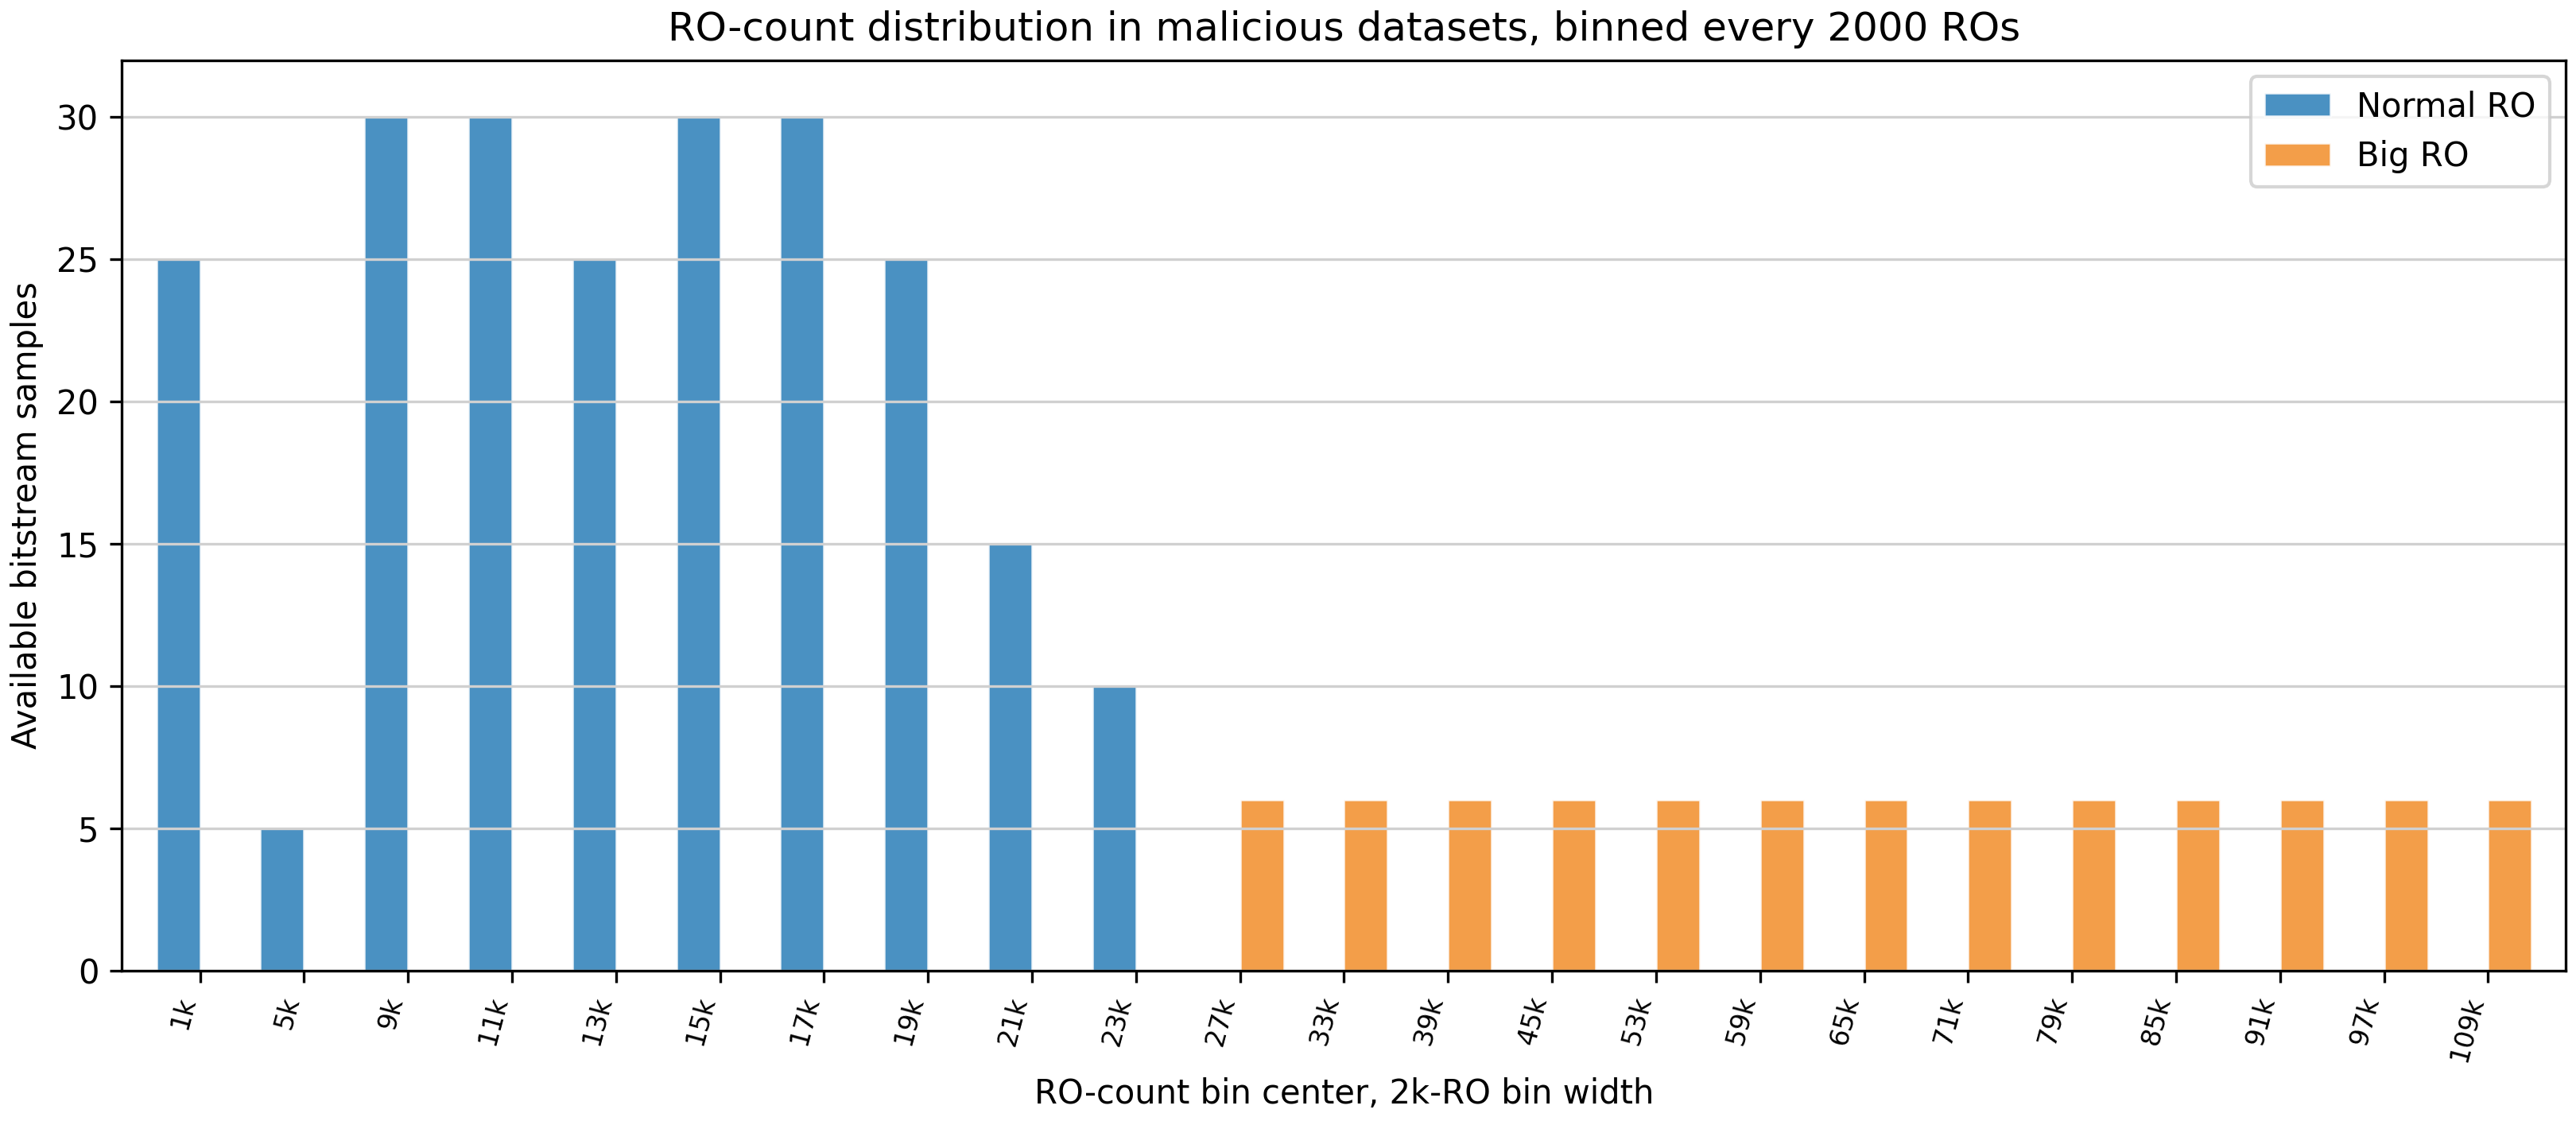
\includegraphics[width=0.95\linewidth]{figures/ro_count_distribution.png}
\caption{Distribution of RO counts in the normal-RO dataset and the big-RO
extension. Bars count available bitstream samples in 2k-RO bins.}
\label{fig:ro-count-distribution}
\end{figure}

\subsection{Preprocessing}
\label{sec:method-preprocessing}

We map each raw partial bitstream to a fixed-size
$H \times W \times 1$ tensor using Algorithm~\ref{alg:preprocessing}. The
transformation uniformly samples or pads the byte stream to $H \cdot W$ bytes,
then inverts, normalizes, and reshapes the selected values.

\begin{algorithm}[t]
\caption{Deterministic bitstream preprocessing.}
\label{alg:preprocessing}
\begin{algorithmic}[1]
\Require Bitstream bytes $b$, target dimensions $H$, $W$
\State $T \gets H \cdot W$
\If{$|b| > T$}
\State $i \gets \left\lfloor \operatorname{linspace}(0, |b|-1, T) \right\rfloor$
\State $b \gets b[i]$
\Else
\State $b \gets \operatorname{ZeroPad}(b, T)$
\EndIf
\State $x \gets \operatorname{Reshape}((255-b)/255, H, W, 1)$
\State \Return $x$
\end{algorithmic}
\end{algorithm}

Our final checker uses a $256 \times 256$ input, corresponding to 65,536 sampled
bytes per partial bitstream. We evaluate additional input resolutions during the
model design-space exploration in Section~\ref{sec:ml-inspection}.


\section{ML-Based Bitstream Inspection}
\label{sec:ml-inspection}

We use convolutional neural networks (CNNs) to classify the fixed-size
bitstream representations introduced in Section~\ref{sec:method-dataset}. Prior work
has shown that bitstream-derived representations contain learnable structure and
can be used to distinguish benign and malicious FPGA designs
\cite{rettkowski2019inspection,chaudhuri2022detection,
elnaggar2023learning,palumbo2022trojan}. CNNs are also well suited to our
deployment goal because quantized models can be translated into FPGA circuits
using tools such as hls4ml~\cite{duarte2018fast,aarrestad2021fast}.

\subsection{CNN Architecture}
\label{sec:cnn-architecture}

The selected checker uses a seven-stage convolutional architecture operating on
a $256\times256$ byte-image tensor. Each stage consists of a quantized
convolution, quantized ReLU activation, and max pooling. Channel width increases
from 8 filters in the first stage to 32 filters in the later stages. A final
average-pooling operation reduces the remaining feature map before a single
quantized dense output produces the classification logit.

Table~\ref{tab:cnn-architecture} summarizes the architecture. We use 8-bit
weights and activations (W8A8) and do not use batch normalization. The output
logit is converted to a maliciousness probability using a sigmoid; the decision
threshold is applied later by the deployment logic.

\begin{table}[t]
\centering
\caption{Seven-stage quantized CNN architecture used by the on-FPGA
checker. All convolutional stages use quantized ReLU activations and W8A8
quantization.}
\label{tab:cnn-architecture}
\small
\begin{tabular}{lcccc}
\toprule
Stage & Filters & Kernel & Stride & Pooling \tabularnewline
\midrule
Conv 0 & 8 & $5\times5$ & $2\times2$ & $2\times2$ \tabularnewline
Conv 1 & 16 & $3\times3$ & $1\times1$ & $2\times2$ \tabularnewline
Conv 2 & 24 & $3\times3$ & $1\times1$ & $2\times2$ \tabularnewline
Conv 3 & 24 & $3\times3$ & $1\times1$ & $2\times2$ \tabularnewline
Conv 4 & 32 & $3\times3$ & $1\times1$ & $2\times2$ \tabularnewline
Conv 5 & 32 & $3\times3$ & $1\times1$ & $2\times2$ \tabularnewline
Conv 6 & 32 & $3\times3$ & $1\times1$ & $2\times2$ \tabularnewline
Output & 1 & -- & -- & AvgPool \tabularnewline
\bottomrule
\end{tabular}
\end{table}

\subsection{Training}
\label{sec:cnn-training}

Models are implemented in TensorFlow~\cite{abadi2016tensorflow} using
QKeras~\cite{coelho2020automatic}. We use quantization-aware training
\cite{coelho2020automatic}, so that the model is trained under the same
fixed-precision behavior used during hardware generation. Training minimizes
binary cross-entropy from logits. We augment the training data with horizontal
and vertical flips and use a balanced production training set containing equal
numbers of benign and malicious samples.

During model development, we use stratified cross-validation to compare model
configurations~\cite{kohavi1995study}. After selecting the final architecture, we train a production
model separately and evaluate it on the held-out test set described in
Section~\ref{sec:eval-setup}.

\subsection{Hardware-Aware Design-Space Exploration}
\label{sec:cnn-design-space}

Model selection considers hardware feasibility in addition to software
classification quality. Rather than exhaustively evaluating every combination
of parameters, we explore the design space in stages. We first vary input
resolution and CNN depth to determine how model capacity and retained bitstream
information affect classification quality. We then evaluate quantization and
pruning as model-compression techniques before passing selected networks to the
hardware synthesis flow described in Section~\ref{sec:on-fpga-checker}.

The principal model-level dimensions are therefore input resolution, network
depth, and numerical precision. Hardware parallelism is explored separately
after conversion to hls4ml by varying operation reuse and per-layer
configuration.

The resulting design-space exploration selects the $256\times256$, seven-layer
W8A8 CNN as the on-FPGA checker used throughout the remainder of the paper.
We also synthesize the same architecture at $512\times512$ to evaluate how
hardware cost scales with input resolution.

\section{On-FPGA Checker}
\label{sec:on-fpga-checker}

We next map the trained bitstream classifier into FPGA logic and consider how
the resulting checker can be placed in the Coyote deployment path. The hardware
design consists of two components: deterministic byte-stream preprocessing and
the quantized CNN classifier. Importantly, both execute on the FPGA, allowing inspection to
take place without a separate host-side classification stage.

\subsection{Hardware Generation}
\label{sec:hardware-generation}

We convert the trained QKeras CNN to hardware using
hls4ml~\cite{duarte2018fast,aarrestad2021fast}. hls4ml translates the quantized
network into an HLS implementation, which is first evaluated through C
simulation and subsequently synthesized to RTL. The final models use
quantization-aware training, so the weight and activation precision used during
training already reflects the W8A8 representation targeted by the generated
hardware.

Before synthesis, we compare the hls4ml C-simulation output against the
corresponding QKeras model. We require matching classifications on the
validation inputs and inspect output deviations before synthesis. This provides
a parity check between the trained model and its fixed-point hardware
implementation.

The preprocessing operation from Section~\ref{sec:method-preprocessing} is
implemented separately in HLS C++ and lowered to RTL. It operates directly on
the incoming bitstream bytes and reproduces the deterministic sampling,
padding, inversion, and normalization used during training. The latency reported
in Section~\ref{sec:eval-hardware} therefore includes both FPGA-side
preprocessing and CNN inference.

\subsection{Hardware Optimization}
\label{sec:hardware-optimization}

Once the trained network is fixed, hls4ml exposes a hardware design space that
trades resource usage against inference latency. The main parameter is the
\emph{reuse factor}, which controls how aggressively arithmetic units are shared
across operations. Lower reuse increases parallelism and reduces latency at the
cost of additional hardware, while higher reuse reduces resource use but
increases execution time.

We initially evaluate resource-oriented hls4ml configurations and sweep reuse
factors for the selected CNN architectures. A single global reuse setting,
however, provides only a coarse tradeoff because convolutional stages differ
substantially in their operation counts and hardware cost. We therefore also
apply manual per-layer reuse settings, assigning greater parallelism to
latency-dominant layers while retaining more sharing elsewhere.

Quantization and pruning are additionally explored as hardware-aware model
transformations. The final checker uses W8A8 quantization trained through
QKeras quantization-aware training. For each transformed model, we retain a
configuration only when software detection quality and hls4ml prediction parity
remain acceptable. Section~\ref{sec:eval-hardware} evaluates the resulting
implementations jointly in terms of detection quality, latency, and routed FPGA
resources.

\subsection{Proposed Coyote Integration}
\label{sec:coyote-integration}

Coyote separates trusted platform services from partially reconfigurable user
regions, providing a natural location for bitstream inspection before
PR~\cite{ramhorst2025coyote}. We propose placing the on-FPGA checker in this
trusted deployment path, as illustrated in
Figure~\ref{fig:coyote-integration}.

An incoming user partial bitstream is first processed by the FPGA-side
preprocessing logic and passed to the synthesized CNN. The CNN produces a
maliciousness score, which trusted deployment logic compares against a configured
threshold. Bitstreams classified as suspicious are rejected, while accepted
bitstreams are allowed to proceed to the Coyote partial-reconfiguration
controller.

\begin{figure*}[t]
\centering
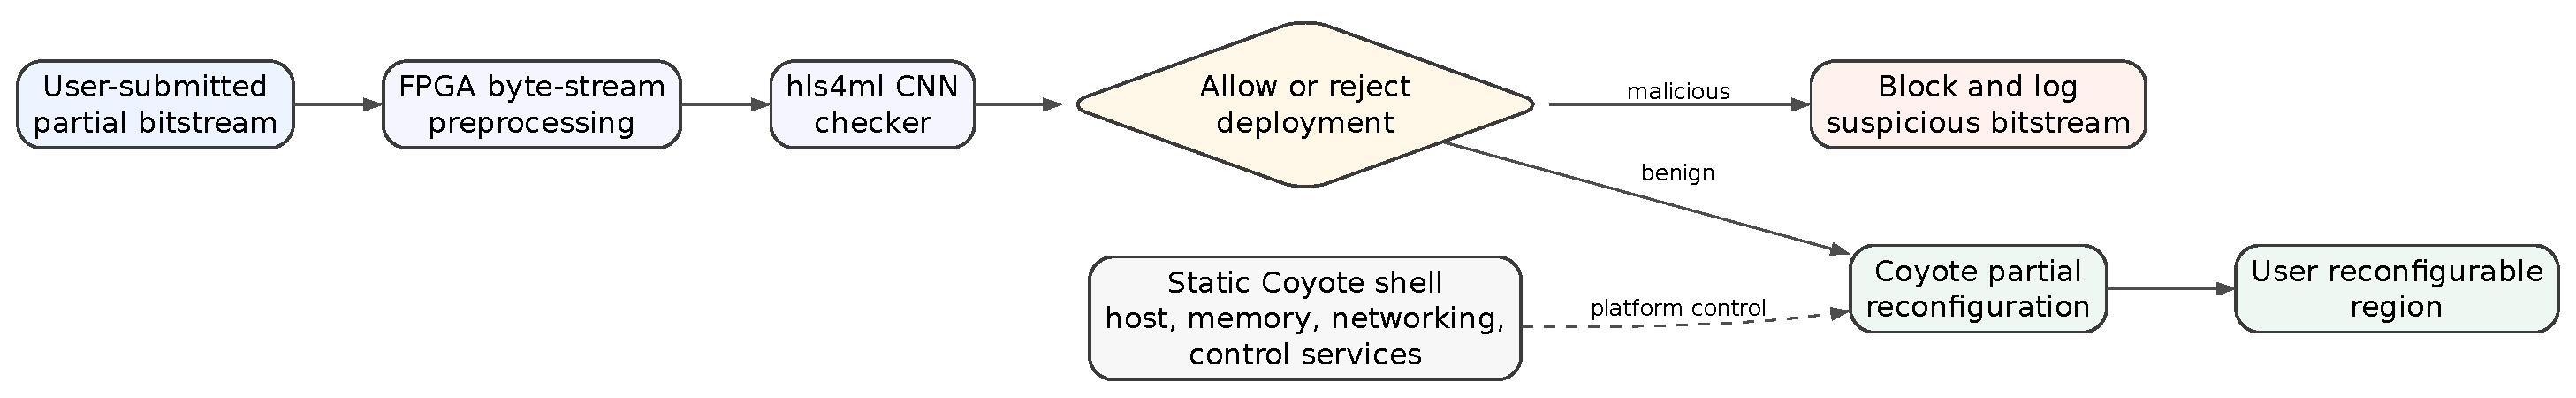
\includegraphics[width=0.95\textwidth]{figures/coyote_integration_path.pdf}
\caption{Proposed integration of the on-FPGA checker into the Coyote
deployment path. FPGA-side preprocessing and CNN inference inspect an
incoming partial bitstream before it is passed to the partial-reconfiguration
controller.}
\label{fig:coyote-integration}
\end{figure*}


The integration shown in Figure~\ref{fig:coyote-integration} is a proposed
deployment architecture rather than a completed end-to-end Coyote
implementation. This work implements and evaluates the FPGA preprocessing and
CNN checker components; connection to Coyote's PR controller and the associated
control-plane logic remain future work.

\section{Evaluation}
\label{sec:evaluation}

We evaluate whether the proposed on-FPGA checker provides useful detection
quality while remaining practical for deployment alongside the Coyote shell and
user logic. In particular, we answer four questions:

\begin{enumerate}
    \item \textbf{Detection quality.} How accurately does the checker
    distinguish benign Coyote partial bitstreams from bitstreams containing
    ring-oscillator (RO) payloads?

    \item \textbf{RO-footprint sensitivity.} How does detection change as the
    malicious RO footprint increases?

    \item \textbf{Hardware feasibility.} What latency and resource overhead does
    the checker introduce on the target FPGA?

    \item \textbf{Deployment-path overhead.} How significant is the added
    inspection latency relative to partial reconfiguration?
\end{enumerate}

Our evaluation considers both the $256^2$- and $512^2$-input, seven-layer
CNNs to characterize the tradeoff between detection quality and hardware cost.
Retaining more bitstream information can improve classification quality, but also
increases latency and on-chip resource requirements. 

\subsection{Experimental Setup}
\label{sec:eval-setup}

We evaluate the checker on the held-out test set defined in
Section~\ref{sec:ml-inspection}. The positive class is the malicious RO class:
a false negative therefore represents a malicious bitstream accepted by the
checker, while a false positive represents a benign accelerator rejected by the
platform. The separate high-density RO set introduced in
Section~\ref{sec:method-dataset} is evaluated only in the RO-footprint analysis.

% TODO: Add the exact benign and malicious sample counts in the held-out test
% set once confirmed from the production manifest.

Predictions use a probability threshold of 0.5, with higher values indicating
greater confidence that a bitstream is malicious. We report accuracy, F1,
true-positive rate (TPR), false-negative rate (FNR), false-positive rate (FPR),
and ROC AUC.

Hardware results target the AMD Alveo U55C. Resource percentages are attributed
to the routed checker hierarchy relative to the complete device. As described in
Section~\ref{sec:on-fpga-checker}, the reported checker latency combines the
FPGA byte-stream preprocessing latency and hls4ml inference latency. It excludes
host-side setup, memory transfers, output readback, logging, and control-plane
operations. Complete integration with Coyote's partial-reconfiguration
controller remains future work.

\subsection{Detection Quality}
\label{sec:eval-detection}

Table~\ref{tab:detection-results} reports the detection quality of the selected
checker on the held-out test set. The model reaches 87.7\% accuracy and an F1
score of 88.5\%. It detects 92.0\% of the malicious bitstreams, corresponding to
an FNR of 8.0\%. Its ROC AUC of 95.1\% indicates that the model provides
substantial separation between the benign and malicious classes across possible
decision thresholds.

\begin{table}[tbp]
    \centering
    \caption{Detection quality of the selected $256^2$-input, seven-layer
    checker on the held-out test set.}
    \label{tab:detection-results}
    \small
    \begin{tabular}{@{}rrrrrr@{}}
        \toprule
        Accuracy & F1 & TPR & FNR & FPR & ROC AUC \\
        \midrule
        87.7\% & 88.5\% & 92.0\% & 8.0\% & 16.9\% & 95.1\% \\
        \bottomrule
    \end{tabular}
\end{table}

The security-relevant error is the FNR because each false negative represents an
malicious bitstream that would pass the checker. At the default threshold,
the model misses 8.0\% of malicious test samples. The corresponding FPR is
16.9\%, meaning that the same operating point rejects a non-negligible fraction
of benign applications.

This trade-off depends on the decision threshold. Reducing the threshold would
reject more malicious bitstreams, but would also block more benign
accelerators. Increasing it would reduce the operational cost of false positives
while admitting more malicious designs. We use threshold 0.5 as a fixed and
reproducible threshold throughout the evaluation. A production deployment
could instead select the threshold according to an explicit platform policy, such
as minimizing the FNR subject to a maximum acceptable FPR.

% Optional figure if an ROC plot is generated.
%
% \begin{figure}[tbp]
%     \centering
%     \includegraphics[width=\columnwidth]{figures/checker_roc.pdf}
%     \caption{ROC curve of the selected on-FPGA checker. The marker shows
%     the operating point produced by probability threshold 0.5.}
%     \label{fig:checker-roc}
% \end{figure}

\subsection{Sensitivity to RO Footprint}
\label{sec:eval-ro-footprint}

Aggregate test-set metrics do not show whether all malicious designs are equally
difficult to detect. We therefore evaluate the checker as a function of the
estimated FPGA footprint occupied by the RO payload. This analysis combines
the standard malicious test samples with the separate high-density RO
extension.

Figure~\ref{fig:ro-footprint} reports the detection rate across  RO LUT
share. Most false negatives occur among the smallest evaluated RO footprints.
As the amount of RO logic increases, the detection rate rises and remains close
to one across the larger footprint ranges. On the high-density extension, the
selected checker reaches a TPR of 98.7\%.

\begin{figure}[tbp]
    \centering
    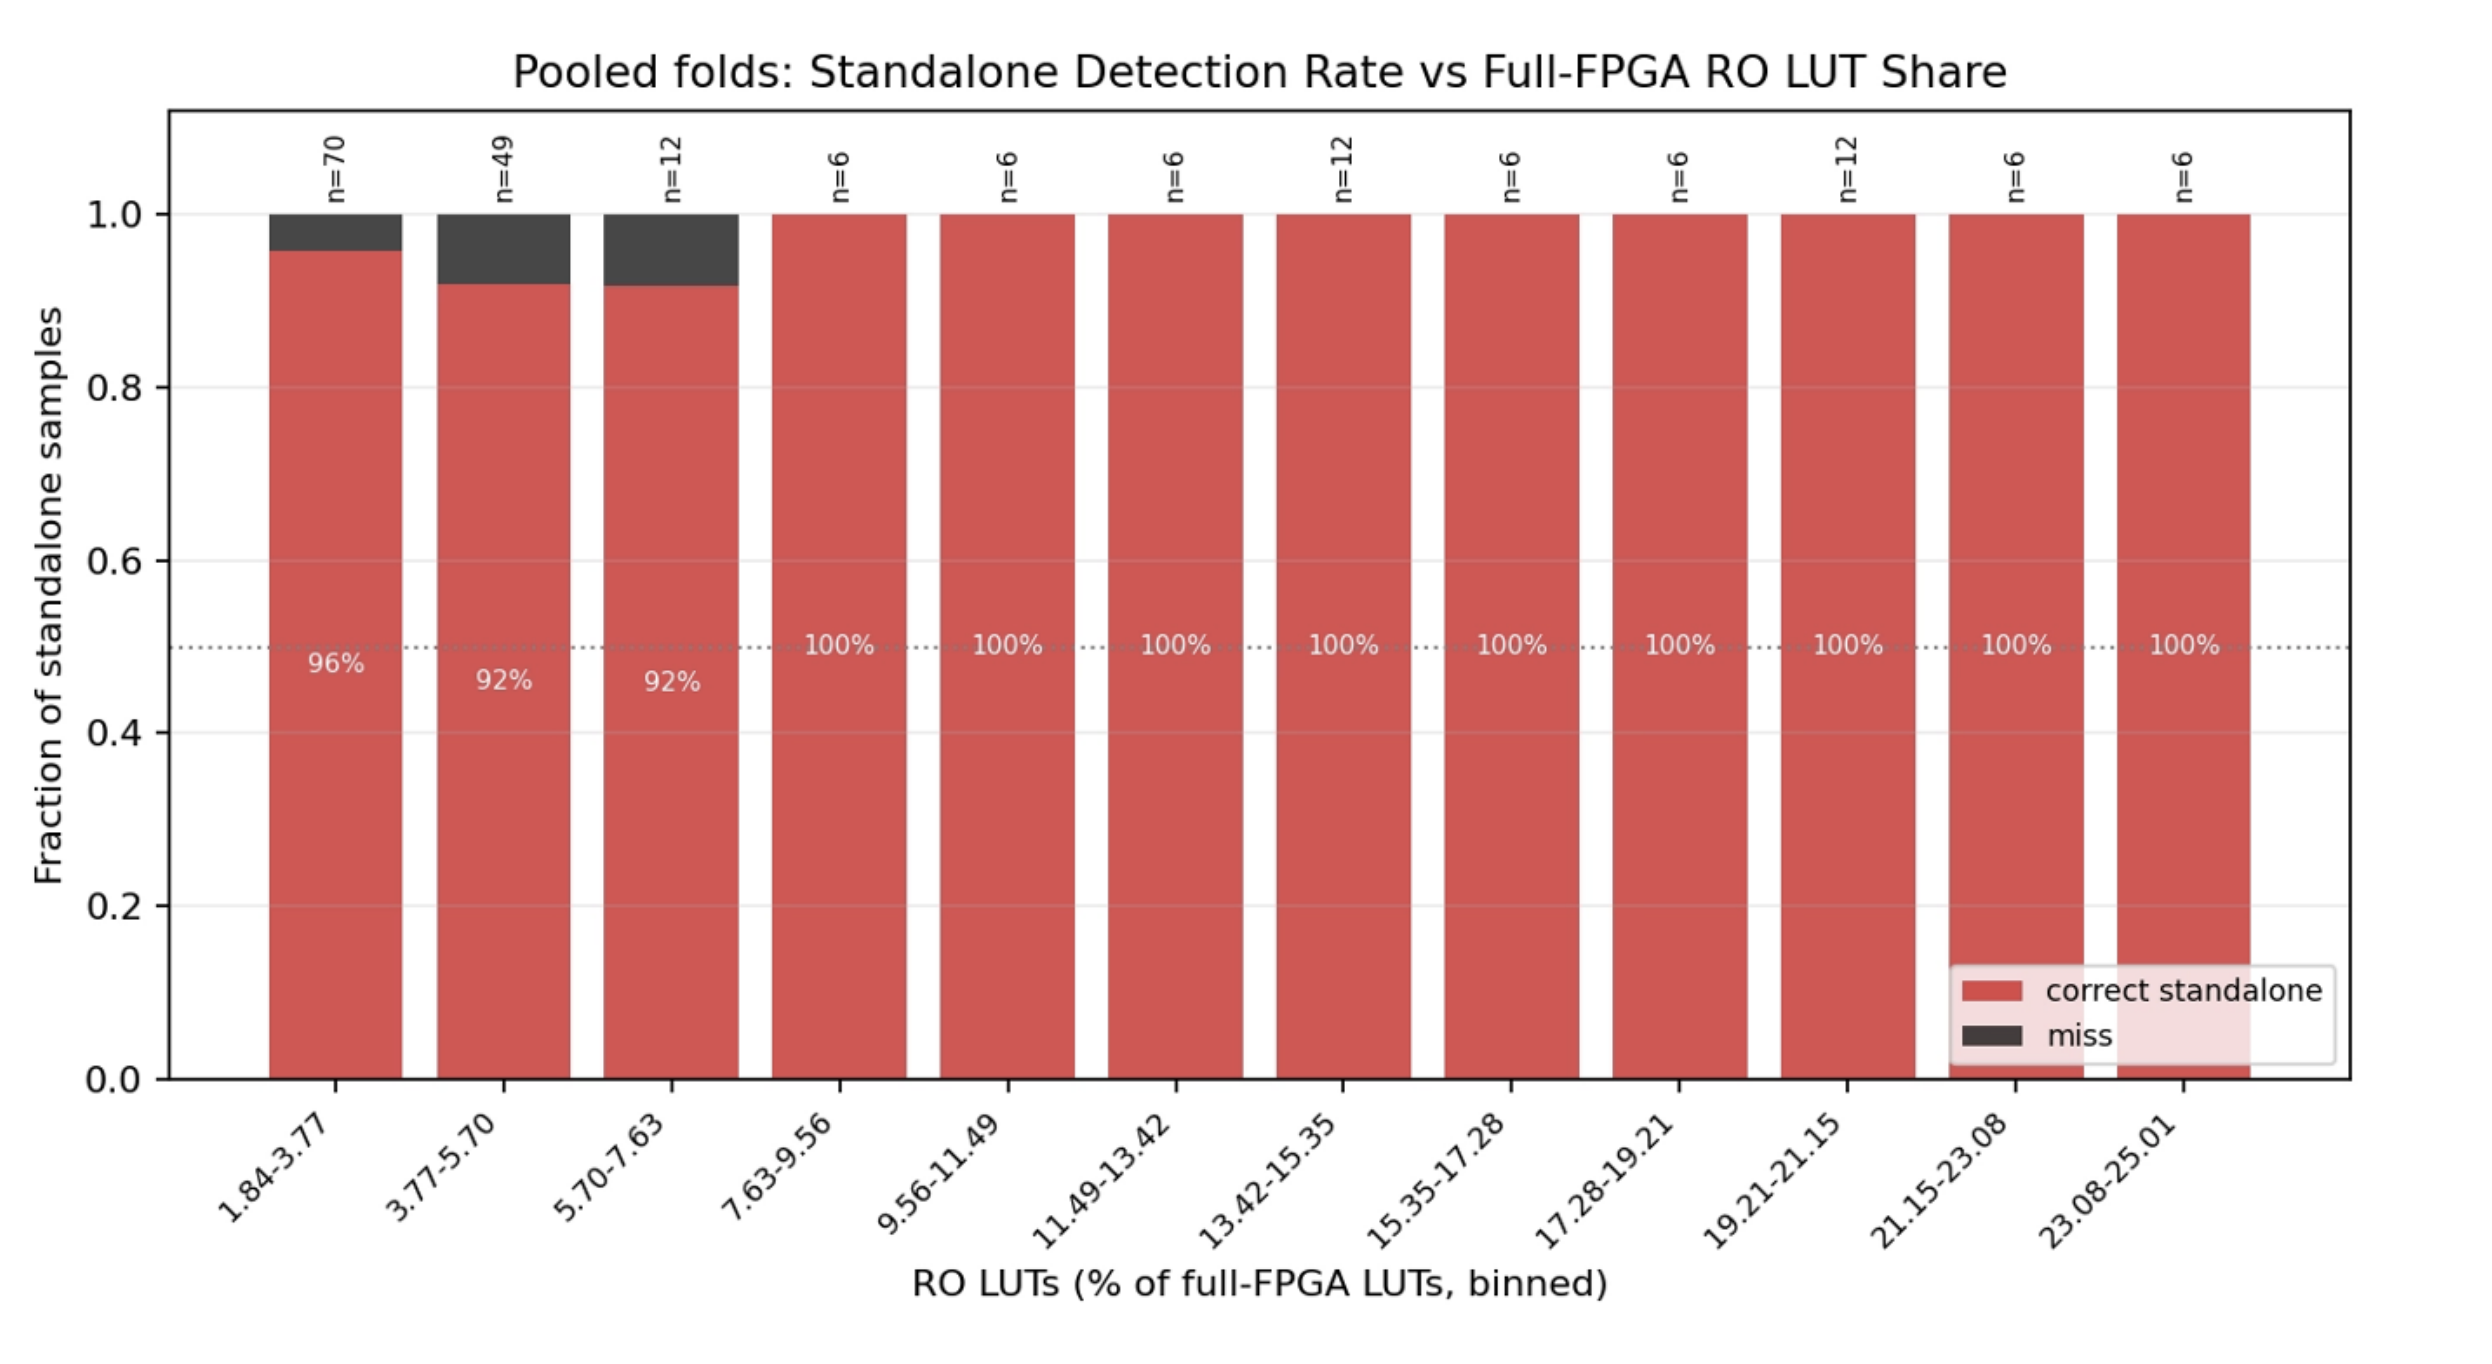
\includegraphics[width=1.1\columnwidth]{figures/ro_footprint_256.png}
    \caption{Detection rate of the selected checker as a function of estimated
    RO LUT share. Misses concentrate among the smallest malicious footprints,
    while larger evaluated RO payloads are detected reliably.}
    \label{fig:ro-footprint}
\end{figure}

This result aligns with demonstrated RO-based attacks, which target availability
through power-hammering and denial of service, or integrity through
voltage-induced fault injection. FPGADefender showed that an optimized design
exceeded the Ultra96 board's power budget using about 3\% of its LUTs and
crashed the board immediately at 5.2\% LUT utilization \cite{la2020fpgadefender}. FPGAhammer induced faults using attacker designs occupying
30--50\% of the available LUTs \cite{fpgahammer2021}, and Mahmoud et al.\ observed
targeted AES faults using tens of thousands of ROs on a cloud-scale FPGA
\cite{mahmoud2023practical}. The checker is therefore strongest in the footprint
range relevant to these demonstrated attacks, while smaller RO payloads for side-channel attacks remain
more difficult to detect.

\subsection{Hardware Evaluation}
\label{sec:eval-hardware}

We convert the selected W8A8 QKeras model using hls4ml. The generated model is
first evaluated through C simulation to confirm consistency with the quantized
software model. We then synthesize the checker and place and route its wrapper
for the Alveo U55C. Manual per-layer reuse settings are used to reduce latency
without adopting the resource cost of a globally latency-optimized
implementation.

Table~\ref{tab:hardware-results} reports the routed resource attribution and
combined preprocessing-plus-inference latency. The selected checker adds 4.47\%
of device LUTs, 17.86\% of BRAM, 1.15\% of URAM, and 14.72\% of DSPs. Its
estimated latency is 3.35\,ms per partial bitstream.

\begin{table}[tbp]
    \centering
    \caption{Routed resource attribution and latency on the Alveo U55C.
    Checker entries are additions to the baseline Coyote shell. The
    $512^2$ implementation is included only as a higher-resolution scaling
    point.}
    \label{tab:hardware-results}
    \small
    \resizebox{\columnwidth}{!}{%
    \begin{tabular}{@{}lrrrrr@{}}
        \toprule
        Design & LUT & BRAM & URAM & DSP & Latency \\
        \midrule
        Baseline Coyote
            & 10.26\% & 9.77\% & 0\% & 0\% & -- \\
        Added $256^2$ checker
            & +4.47\% & +17.86\% & +1.15\% & +14.72\% & 3.35\,ms \\
        Added $512^2$ checker
            & +4.90\% & +61.78\% & +1.77\% & +14.45\% & 6.53\,ms \\
        \bottomrule
    \end{tabular}%
    }
\end{table}

The selected design fits alongside the baseline shell, although its BRAM and DSP
requirements are substantial. LUT use remains moderate, while BRAM is the most
important resource constraint. After adding the checker, memory resources must
still remain available for platform services and user accelerators. This makes
the memory footprint more significant than the comparatively small LUT
increase.

Figure~\ref{fig:f1-resolution-depth} summarizes the software design space that
motivates the hardware comparison. Detection quality generally improves as the
input resolution and CNN depth increase. The seven-layer models achieve the
strongest pooled-validation results, while the gains from increasing resolution
become smaller at the largest configurations. These results motivate evaluating
whether the additional detection quality of larger models justifies their hardware
cost. The values in this figure are pooled-validation results used for model
selection and are therefore distinct from the held-out test results reported in
Table~\ref{tab:detection-results}.

\begin{figure}[tbp]
    \centering
    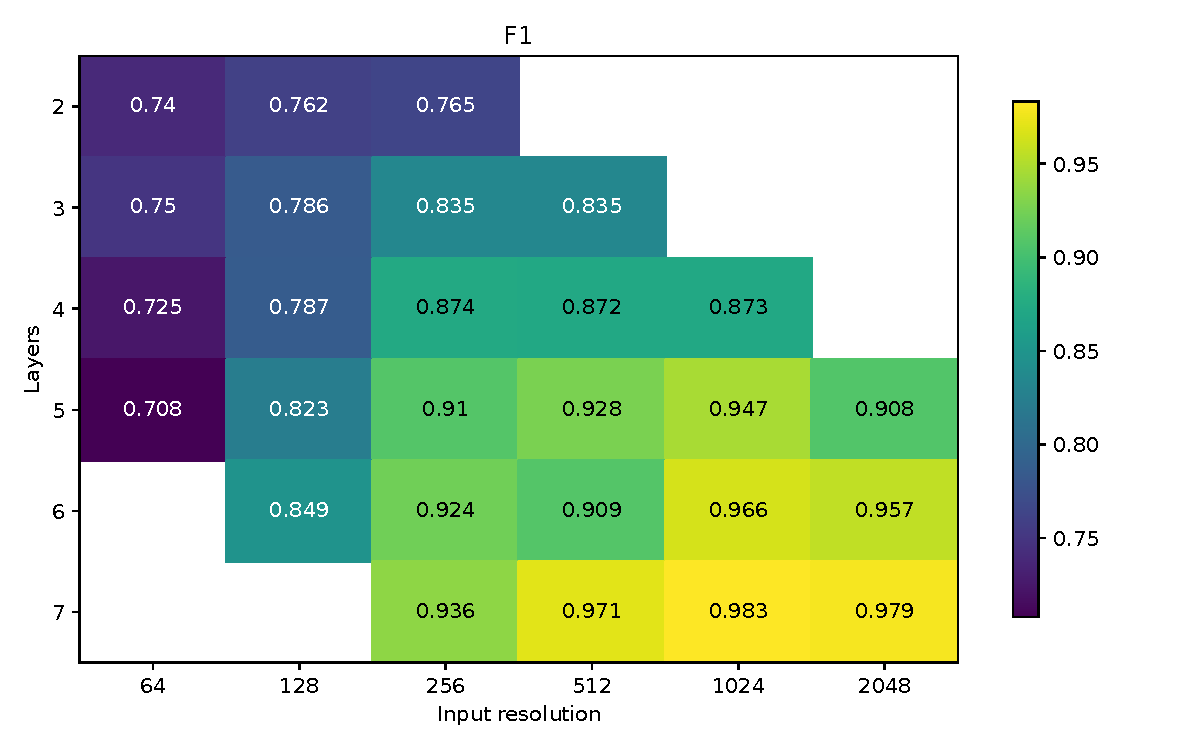
\includegraphics[width=1.1\columnwidth]{figures/f1_resolution_depth.pdf}
    \caption{Pooled-validation F1 across input resolution and CNN depth.
    Detection quality generally improves with larger inputs and deeper models.}
    \label{fig:f1-resolution-depth}
\end{figure}

To examine scaling, we also synthesize the same seven-layer architecture with a
$512 \times 512$ input. This configuration retains four times as many sampled
bytes as the selected checker. It improves F1 from 88.5\% to 90.5\%, but nearly
doubles the checker latency from 3.35\,ms to 6.53\,ms. More importantly, its
attributed BRAM use rises from 17.86\% to 61.78\% of the complete device.

The higher-resolution result demonstrates that model scaling quickly becomes
impractical. The small improvement in classification quality requires more than
three times the BRAM of the selected checker and leaves limited memory capacity
for the shell, platform functionality, and user logic. We therefore treat the
$512^2$ implementation as evidence of the hardware scaling limit rather than as
a deployment candidate.

Figure~\ref{fig:hardware-frontier} places the selected checker in the broader
hardware design space. Increasing input resolution and reducing operation reuse
can improve detection quality or latency in isolation, but moves the design
toward higher resource consumption. Per-layer tuning shifts the selected
$256^2$ checker toward a more useful operating point. The resulting model
retains useful detection quality while avoiding the rapid BRAM growth of the
higher-resolution implementation.

\begin{figure}[tbp]
    \centering
    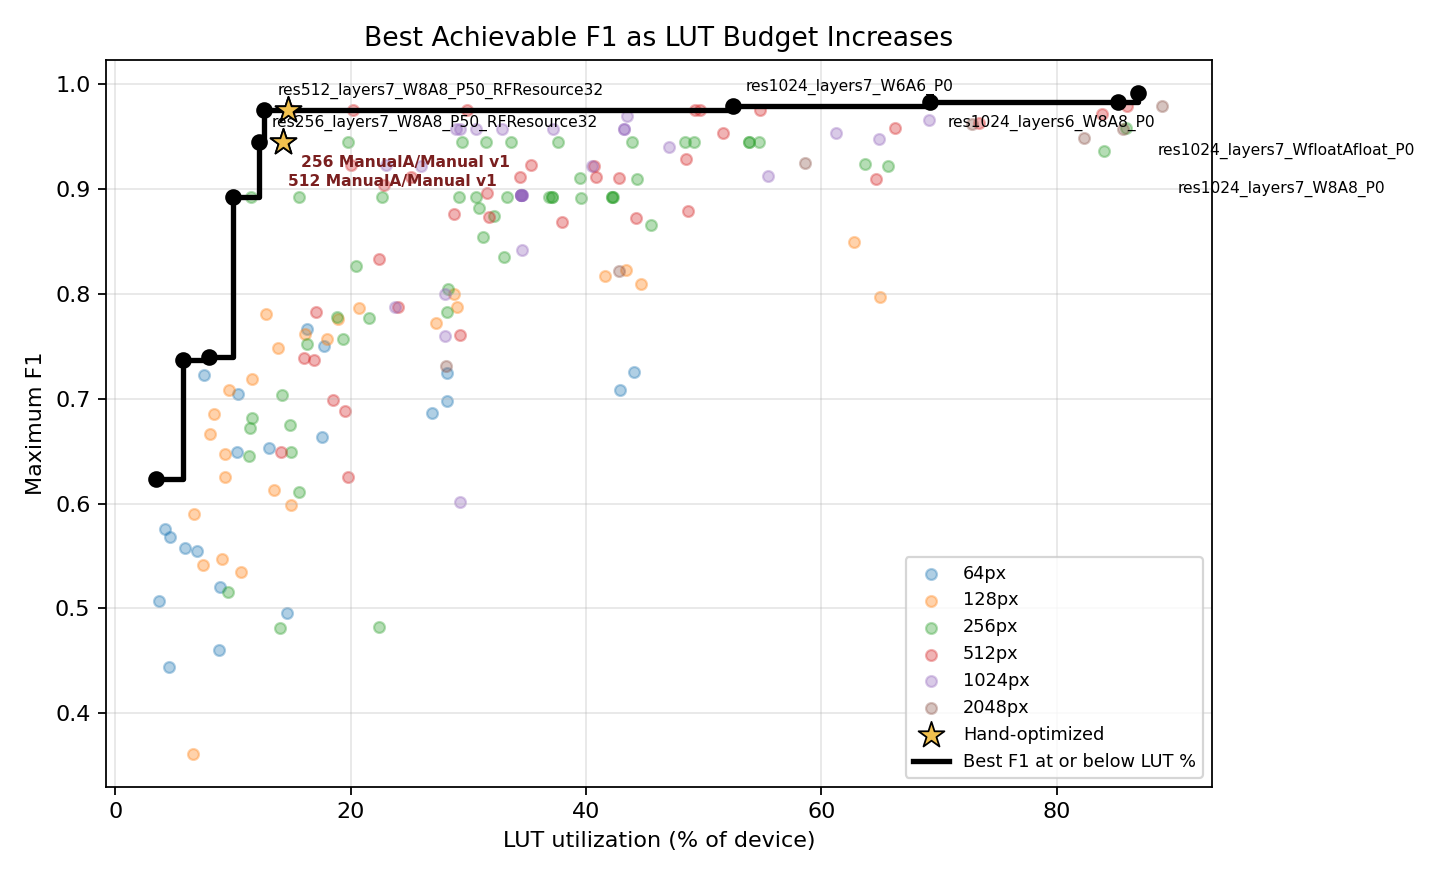
\includegraphics[width=1.15\columnwidth]{figures/hls_lut_f1_frontier.png}
    \caption{F1 versus LUT utilization across synthesized candidates. The black
curve shows the best-achievable F1 frontier, while stars mark the hand-optimized
$256^2$ and $512^2$ designs.}

    \label{fig:hardware-frontier}
\end{figure}

\subsection{Deployment-Path Overhead}
\label{sec:eval-deployment}

Inspection is performed before partial reconfiguration and therefore adds to the
deployment latency of each submitted bitstream. Table~\ref{tab:pr-overhead}
compares the selected checker's 3.35\,ms latency with previously reported Coyote
partial-reconfiguration measurements.

\begin{table}[tbp]
    \centering
    \caption{Estimated overhead of the selected checker relative to previously
    reported Coyote partial-reconfiguration latency
    \cite{korolija2020os}.}
    \label{tab:pr-overhead}
    \small
    \begin{tabular}{@{}lrrr@{}}
        \toprule
        PR region & PR latency & Checker & Overhead \\
        \midrule
        6\%  & 6.04\,ms  & 3.35\,ms & 55.5\% \\
        33\% & 36.94\,ms & 3.35\,ms & 9.1\% \\
        66\% & 73.27\,ms & 3.35\,ms & 4.6\% \\
        \bottomrule
    \end{tabular}
\end{table}

For a small 6\% reconfigurable region, inspection adds more than half of the
reference PR latency. The relative cost falls to 9.1\% for a 33\% region and
4.6\% for a 66\% region. The checker is therefore most attractive for
deployments in which the reconfiguration itself already takes tens of
milliseconds. Its cost is more pronounced for small regions with short
reconfiguration times.

These comparisons provide deployment context rather than an end-to-end
measurement of an integrated system. The reported 3.35\,ms covers FPGA-side
preprocessing and inference but excludes command handling, buffering, logging,
threshold-policy enforcement, and transfer of an accepted bitstream to the PR
controller. Full integration may therefore add further fixed overhead.

Overall, the $256^2$ seven-layer CNN is the selected design point. It reaches
88.5\% F1 with an 8.0\% false-negative rate, detects 98.7\% of the separate
high-density RO samples, and completes preprocessing and inference in an
estimated 3.35\,ms. Its resource footprint is compatible with feasibility on the
U55C, while the higher-resolution experiment shows that increasing model input
size rapidly becomes constrained by BRAM and latency. These results support
the feasibility of an on-FPGA checker for RO-focused, defense-in-depth
inspection before partial reconfiguration.

\section{TODO: Discussion + Conclusion}

\bibliographystyle{ACM-Reference-Format}
\bibliography{sample-base}

\end{document}
\endinput
%%
%% End of file `sigconf.tex'.
